%%% LaTeX Template: Article/Thesis/etc. with colored headings and special fonts
%%%
%%% Source: http://www.howtotex.com/
%%% Feel free to distribute this template, but please keep to referal to http://www.howtotex.com/ here.
%%% February 2011
%%%
%%% Last updated September 2018 by CDM

%%%  Preamble
\documentclass[11pt,letterpaper]{article}
\usepackage[margin=1.0in]{geometry}
\usepackage[T1]{fontenc}
\usepackage[bitstream-charter]{mathdesign}
\usepackage[latin1]{inputenc}					
\usepackage{amsmath}						
\usepackage{xcolor}
\usepackage{cite}
\usepackage{hyphenat}
\usepackage{graphicx}
\usepackage{float}
\usepackage{subfigure}
\usepackage{sectsty}
\usepackage[compact]{titlesec} 
\usepackage[tablegrid]{vhistory}
\allsectionsfont{\color{accentcolor}\scshape\selectfont}

%%% Definitions
%%%%%%%%%%%%%%%%%%%%%%%%%%%%%%%%%%%%%%%%%%%%%%%%%%
% Change me to fit your team/semester information
\definecolor{accentcolor}{rgb}{0.0,0.0,0.5} 
\newcommand{\teamname}{Gamma}
\newcommand{\productname}{IEEE robotics competition region 5 2022}
\newcommand{\coursename}{CSE 4316: Senior Design I}
\newcommand{\semester}{Fall 2021}
\newcommand{\docname}{Project Charter}
\newcommand{\department}{Department of Computer Science \& Engineering}
\newcommand{\university}{The University of Texas at Arlington}
\newcommand{\authors}{Evan Cornish \\ Kartikey Sharan \\ Zachary Trumbaturi \\ Osama Siddiqui \\ Paola Gonzalez}

%%% Headers and footers
\usepackage{fancyhdr}
	\pagestyle{fancy}						% Enabling the custom headers/footers
\usepackage{lastpage}	
	% Header (empty)
	\lhead{}
	\chead{}
	\rhead{}
	% Footer
	\lfoot{\footnotesize \teamname \ - \semester}
	\cfoot{}
	\rfoot{\footnotesize page \thepage\ of \pageref{LastPage}}	% "Page 1 of 2"
	\renewcommand{\headrulewidth}{0.0pt}
	\renewcommand{\footrulewidth}{0.4pt}

%%% Change the abstract environment
\usepackage[runin]{abstract}			% runin option for a run-in title
%\setlength\absleftindent{30pt}			% left margin
%\setlength\absrightindent{30pt}		% right margin
\abslabeldelim{\quad}	
\setlength{\abstitleskip}{-10pt}
\renewcommand{\abstractname}{}
\renewcommand{\abstracttextfont}{\color{accentcolor} \small \slshape}	% slanted text

%%% Start of the document
\begin{document}

%%% Cover sheet
%%%%%%%%%%%%%%%%%%%%%%%%%%%%%%%%%%%%%%%%%%%%%%%%%%%%%%%%%%%%%%%%%%%%%%%%%%%%
%   CHANGE THE GRAPHIC HERE. PUT YOUR IMAGE IN THE 'images' 
%   FOLDER AND UPDATE THE NAME FROM 'images/test_image' TO YOUR IMAGE NAME
{\centering \huge \color{accentcolor} \sc \textbf{\department \\ \university} \par}
\vspace{1 in}
{\centering \huge \color{accentcolor} \sc \textbf{\docname \\ \coursename \\ \semester} \par}
\vspace{0.5 in}
% Begin image insertion ----------------
\begin{figure}[h!]
	\centering
   	
\includegraphics[width=0.60\textwidth]{images/team_gamma} % Change image name
\end{figure}
% End image insertion ------------------
\vspace{0.5 in}
{\centering \huge \color{accentcolor} \sc \textbf{\teamname \\ \productname} \par}
\vspace{0.5 in}
{\centering \large \sc \textbf{\authors} \par}
\newpage


%\vspace{1 in}
%\centerline{January 13th, 2012}
%\newpage

%%% Revision History
%%%%%%%%%%%%%%%%%%%%%%%%%%%%%%%%%%%%%%%%%%%%%%%%%%%%%%%%%%%%%%%%%
% Each '\vhEntry' begins a new version entry, and each {} is a 
% column. Update this to reflect your version history.
\begin{versionhistory}
  	\vhEntry{0.1}{10.11.2021}{EC|OS|ZT|KS|PG}{document creation}
\end{versionhistory}
\newpage

%%% Table of contents
\tableofcontents
\newpage

%%% List of figures and tables (optional)
\listoffigures
%\listoftables
\newpage
\setcounter{table}{0}

%%% Executive summary sections
% The \section command creates a section, assigns it a number and gives it the title in the braces.
% The \input command inserts the contents of the text file indicated in the braces.
\section{Problem Statement}
Our reason for creating an underwater, remote-controlled robot is to compete in the IEEE Region 5 Robotics Competition. Every day, 2 million tons of sewage and industrial and agricultural waste are discharged into the world's water (UN WWAP 2003), the equivalent of the weight of the entire human population of 6.8 billion people. Water pollution is a major problem in today's world, which can have dire consequences. The objective of the competition is to demonstrate the use of a tethered underwater robot to collect 'trash' from the ocean floor, midwater, and surface. The robot then will deposit the trash in a proper receptacle. The game field simulates an underwater environment containing objects such as industrial infrastructure and underwater debris. Underwater and surface obstacles and anomalies represent typical operational challenges. 
\section{Methodology}
The team is working diligently to build a tethered underwater robot that will collect trash from ocean floor, midwater, and surface. The team will mitigate the given problem statement by implementing a robot with thrusters and ballast tanks to master basic movements such as forward, backward, and sideways motion. The team will further perfect the robot's maneuvers by mounting an ethernet camera to see and avoid obstacles in real time. Additionally, the team will install certain mechanisms on the robot to aid the process of trash collection. Finally, the robot will make use of the thrusters and camera to rise to the ocean floor and accompanied by another mechanism it will be able to place the collected trash in a proper receptacle.  

 

Assumptions  

 
\begin {enumerate}
	\item A suitable outdoor or indoor testing location (swimming pool) will be available by the 3rd sprint cycle. 

	\item The delivery of ordered materials and components will be made by Amazon and other vendors by 4th sprint cycle. 

	\item Access to 3-D printer will be available, to print parts for robot's frame, throughout 3rd and 4th sprint cycle.  

	\item The buoyancy calculation for Trash to be collected by robot will hold true upon initial testing of trash collection mechanism.  

	\item Access to thrusters and Raspberry Pi will be available through Dr. McMurrough and Professor Conly by 3rd sprint cycle. 
\end{enumerate}
\section{Value Proposition}
With the creation of this project, we are fighting for a greater cause. It will help clean up our oceans, which has been destroyed by oil spills and industrial pollution. This is a growing problem that is spreading each day and endangering the animals that live there. That is why constant experimentation on ways to pick up all this trash is crucial. Even if we fail in creating a working robot, this project will help gain insight in new, even cheaper, faster ways to clean up pollution in the water. This could also be a valuable lesson for students to show them how hard it is to clean up garbage, especially when the oceans are so infested with it.
\section{Development Milestones}
This list of core project milestones should include all major documents, demonstration of major project features, and associated deadlines. Any date that has not yet been officially scheduled at the time of preparing this document may be listed by month.
\\
\\
Provide a list of milestones and completion dates in the following format:
%%%%%%%%%%%%%%%%%%%%%%%%%%%%%%%%%%%%%%%%%%%%%%%%%%%%%%%%%%%%%%%%%%%%%%%%%
% This creates a bullet list. To add a bullet, use the \item command.
% Make sure it is between the \begin{itemize} and \end{itemize} commands.
\begin{itemize}
  \item Project Charter first draft - October 2021
  \item System Requirements Specification - October 2021
  \item Architectural Design Specification - November 2021
  \item Demonstration of propulsion and diving movement - December 2021
  \item Detailed Design Specification - December 2021
  \item Demonstration of driving and controlled movement - January 2022
  \item Demonstration of robotic arm/grasping mechanism - January 2022
  \item CoE Innovation Day poster presentation - April 2022
  \item Demonstration of tennis ball collection - February 2022
  \item Demonstration of tennis ball deposit/launch - March 2022
  \item Demonstration of speed improvements - March 2022
  \item Final Project Demonstration - April 2nd 2022
\end{itemize}
\newpage

%%% Remaining project charter sections
\section{Background}
Currently, robots exist that are intended to collect waste from the surface of water. A few examples of these types of robots are WasteShark \cite{global} and Urban Rivers \cite{asme}. However, there are no functional robots currently, that can collect waste and debris from the ocean floor and midwater. Our goal is to create a robot that can collect trash from the surface, midwater, and ocean floor. This is important since large quantities of trash accumulate on the ocean floor, which poisons fishes and other marine animals. If a product like ours is successful, it can be adopted by many governments and firms to cleanse their water bodies, and improve the quality of water. 
\section{Related Work}
Given that this is a robotics competition there are no state of the art solutions that would be acceptable to use. There is one tethered robot that from QYSEA called the fifish-v6 \cite{GYSEA}. This will be the inspiration for our design but no components will be copied except for general position of the thrusters and the number of thrusters to use.

%%%%%%%%%%%%%%%%%%%%%%%%
% To cite something, use the \cite command with the name of the bibtex entry in the curly braces.
% It will determine which reference number it is and insert that number where the \cite command is.
% e.g. \cite{Rubin2012}
\section{System Overview}
Our system will consist of a carbon fiber frame, either 6 underwater electric thrusters or a combination of 2 thrusters and 4 ballast tanks, a pulley powered cannon for shooting tennis balls and a mechanical arm for grasping items with a camera attached to the end. 
The carbon fiber frame will need to be held together by 3d printed connecting parts. In addition, we will need at least 2 but possibly more Arduino boards to connect to the thrusters for the purpose of switching them on and off. The Arduinos will receive input from a Raspberri pi 4 that will send the signals based on a driver directing the robot. The Raspberri pi will also receive the camera feed from the front arm of the robot.


\begin{figure}[h!]
	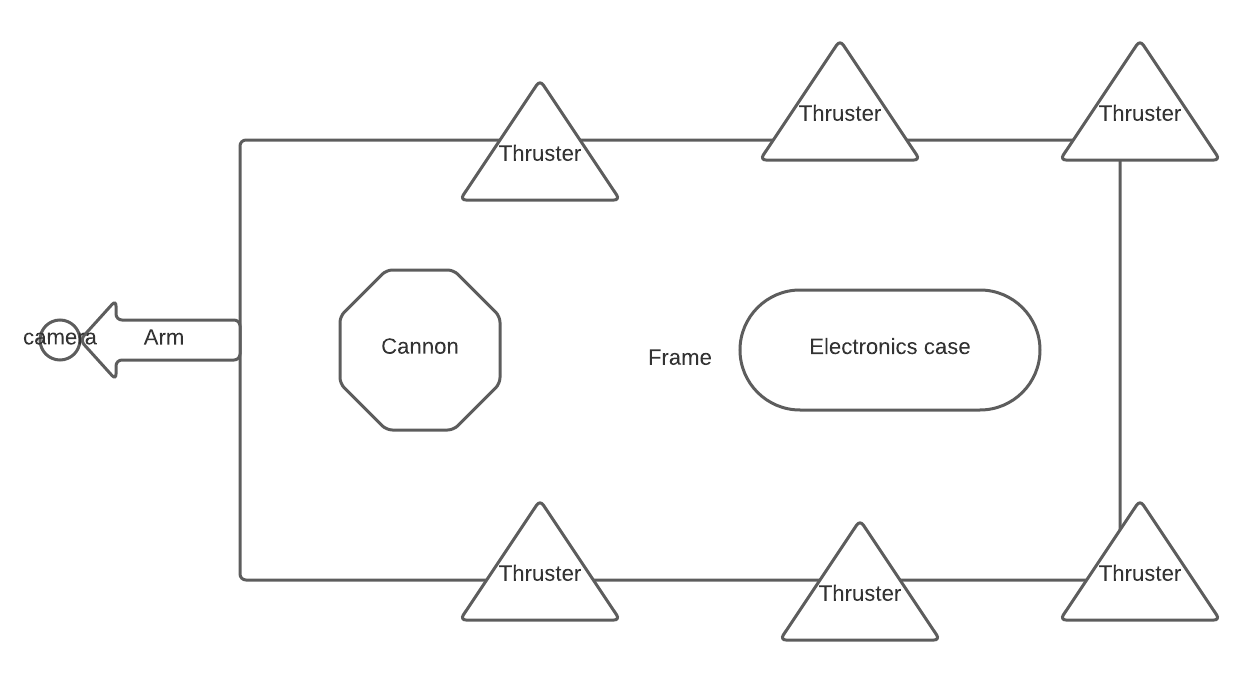
\includegraphics{images/initial_diagram.png}
\end{figure}
\section{Roles \& Responsibilities}
The project owner and scrum master will change periodically to give everyone a chance for the role. The stakeholders in this project are the judges for the IEEE Robotics competition. They will give or remove points on our robot based on the rules of the competition, just like how a customer will rate the worker based on how well their needs were met. Dr. McMurrough will be our point of contact. Our group members consist of Kartikey, Osama, Paola, Evan and Zach. We have assigned individual tasks for everyone. Kartikey and Osama will learn 3D modeling for potential corner pieces or other custom parts. Evan, Paola and Zach are Learning Arduino coding standards for basic thruster movement. As a group, we will blueprint a basic frame for the robot, secure a testing site for the robot, and when parts arrive, meet with Dr. McMurrough to discuss more possible ideas for basic mechanisms.
\section{Cost Proposal}
Currently as this is consisting of the first round of parts, the group was conservative with their purchasing with the initial budget of \$800.00. The Arduino was needed as a basic microcontroller to handle future thruster implementation. Dr. McMurrough has thrusters that he will lend for the project, so the microcontroller will be able to interface directly into those. Expansions to the microcontroller could be needed like an I2C bus for more inputs, but that is undetermined at this time. Next the chosen frame was to make it out of glossy carbon fiber tubing. Six total pieces were purchased to give the group the initial flexibility to create a basic frame to mount components to. The pelican watertight case was another recommendation by Dr. McMurrough to hold the electronics and keep them safe. Possible weights or concerns of density will be addressed when the parts arrive.



\subsection{Preliminary Budget}
\begin{table}[H]
	\resizebox{\textwidth}{!}{
		\begin{tabular}{|l|l|l|}
			\hline
			\textbf{Purchased Item} & \textbf{Quantity} & \textbf{Cost} \\ \hline
			Arduino Uno R3  & 1 & \$13.99 \\ \hline
			Carbon Fiber Tube 16mm x 14mm x 500mm (2 Pieces)  & 3 & \$56.85  \\ \hline
			Pelican 1200 Case With Foam & 1 & \$52.72 \\ \hline
			Total Cost: & - & \$123.56 \\ \hline
	\end{tabular}}
	\caption{Breakdown of Current Costs} 
\end{table}



\subsection{Current \& Pending Support}
Senior Design Standard Budget \$800.00 - This is given to all senior design teams to use for the progression of their project. Since this project is hardware based, it is possible that this budget could increase if the need arises, but for now the budget is firm \$800.00.
\section{Facilities \& Equipment}
Since this robot is required to work underwater, we will need a pool of some sort to test it out. The pool must be large enough and deep enough to put stuff in and for our robot to move around in. Its possible we can just buy a pool or contact someone who has a pool that we can use. Another thing we need is a 3D printer to create custom parts. We will be using the application Tinkercad for 3D modeling. The parts for the robot will be purchased online. We have put together a list of equipment that we will start out with and add more things to the list as project testing continues. We will need 6 pieces of carbon fiber tubing, which will be the basis for the frame. Another thing we need is a pelican case, a watertight container to hold our electronics. Lastly, we will need an Arduino Uno R3, a microcontroller we might change in the future for more outputs. One thing we are on the fence on is if we should get Ballast tanks or thrusters. We're leaning more on thrusters as they are easier to use and have more accessible.
\section{Assumptions}
An assumption is a belief of what you assume to be true in the future. You make assumptions based on your knowledge, experience or the information available on hand. These are anticipated events or circumstances that are expected to occur during your project's life cycle.

Assumptions are supposed to be true but do not necessarily end up being true. Sometimes they may turn out to be false, which can affect your project significantly. They add risks to the project because they may or may not be true. For example, if you are working on an outdoor unmanned vehicle, are you assuming that testing space will be available when needed? Are you relying on an external team or contractor to provide a certain subsystem on time? If you are working at a customer facility or deploying on their computing infrastructure, are you assuming you will be granted physical access or network credentials?

This section should contain a list of at least 5 of the most critical assumptions related to your project. For example:

The following list contains critical assumptions related to the implementation and testing of the project.

%%%%%%%%%%%%%%%%%%%%%%%%%%%%%%%%%%%%%%%%%%%%%%%%%%%%%%%%%%%%%%%%%%%%%%%%%
% This creates a bullet list. To add a bullet, use the \item command.
% Make sure it is between the \begin{itemize} and \end{itemize} commands.
\begin{itemize}
  \item A suitable outdoor testing location will be available by the 3rd sprint cycle
  \item The X sensing system developed by Sensor Consulting Company will be delivered according to specifications by the 4th sprint cycle
  \item Access to the customer installation site will be provided by the 5th sprint cycle
  \item The customer will provide ample power and network connectivity at the installation site
  \item The installation site network infrastructure will allow TCP network traffic on port 8080
\end{itemize}
\section{Constraints}
12 Constraints
----------------------

The following list contains key constraints related to the implementation and testing of the project.



%%%%%%%%%%%%%%%%%%%%%%%%%%%%%%%%%%%%%%%%%%%%%%%%%%%%%%%%%%%%%%%%%%%%%%%%%
% This creates a bullet list. To add a bullet, use the \item command.
% Make sure it is between the \begin{itemize} and \end{itemize} commands.
\begin{itemize}
	\item Competition is on April 2, 2020, so the project must have all major adjustments and design elements ready about a week before due to workshop being in Arlington versus the competition in Houston.
	\item Amazon shipping can take a little bit of time after ordering with the support ticket. 
	\item Must be able to balance projects in other classes simultaneously with the senior design project.
	\item Total development costs must not exceed \$800 (for now).
	\item Coordination between teammates developing their respective modules must work seemlessly.
\end{itemize}
\section{Risks}
13 - Risks
-----------------------------------

The following high-level risk census contains identified project risks with the highest exposure. Mitigation strategies will be discussed in future planning sessions.



%%%%%%%%%%%%%%%%%%%%%%%%%%%%%%%%%%%%%%%%%%%%%%%%%%%%%%%%%%%%%%%
% This is the table. To add a row, separate each column with an
% ampersand (&) and end the line with the \hline command.
\begin{table}[H]
	\resizebox{\textwidth}{!}{
		\begin{tabular}{|l|l|l|l|}
			\hline
			\textbf{Risk description} & \textbf{Probability} & \textbf{Loss (days)} & \textbf{Exposure (days)} \\ \hline
			Further delay for arrival of ordered parts on top of standard shipping delay  & 0.30 & 8 & 2.4 \\ \hline
			No testing environment (a pool) is available for use  & 0.10 & 2 & 0.2 \\ \hline
			Possibility of shorted parts and need to order replacements  & 0.50 & 9 & 4.5 \\ \hline
			Chosen laptop for controlling robot in competition breaks down & 0.05 & 20 & 1 \\ \hline
			Robot cannot stay together using chosen bonding materials and brackets & 0.20 & 4 & 0.8 \\ \hline
	\end{tabular}}
	\caption{Overview of highest exposure project risks} 
\end{table}
\section{Documentation \& Reporting}
%%% In this section, you will describe all of the various artifacts that you will generate and maintain during the project life cycle. Describe the purpose of each item below, how the content will be generated, where it will be stored, how often it will be updated, etc. Replace the default text for each section with your own description. Reword this paragraph as appropriate.

\subsection{Major Documentation Deliverables}


\subsubsection{Project Charter}
This document will be updated at the end of each sprint, since that is when we will update our design, risks, costs, and other items included in the project charter. The initial version will be delivered on $11^{th}$ October 2021. The final version will be delivered at the end of November or early December. 

\subsubsection{System Requirements Specification}
This document will be updated if we make changes to the core functionality of the robot. This seems unlikely, since the robot will adhere to the rules of the robotics competition. The initial version will be delivered on $25^{th}$ October 2021. The final version will be delivered at the end of the semester 

\subsubsection{Architectural Design Specification}
This document will be updated if changes are made to the overall design of the robot. Initial version will be delivered on $15^{th}$ November 2021. The final version will be delivered at the end of the semester 

\subsubsection{Detailed Design Specification}
This document will be updated once we have specific details of the robot, and its mechanisms. Any minor changes made to the robot will be recorded. The initial and final version will be delivered at the end of the semester. 

\subsection{Recurring Sprint Items}


\subsubsection{Product Backlog}
Evan Cornish will be responsible for the task of maintaining the product backlog. Each sprint the tasks that are completed will be reported in the group meetings, and the tasks will be moved ot the completed section.
Our backlog will be maintained on the Jira software. Backlog items will be added and marked complete by a group vote. 

\subsubsection{Sprint Planning}
There will be a meeting every 2 weeks solely for sprint planning purposes. At this meeting tasks that need to be accomplished will be voted upon, and then responsibilities will be assigned based on a group decision as well.
There are 5 remaining sprints available during the Fall semester not counting winter break. Over winter break our goal is to do 1 more sprint, taking 1 week off for Christmas.
There are 5 sprints available before the competition date of April 2nd. That means our total remaining sprints is 11 or 12 depending on how many we manage over winter break.

\subsubsection{Sprint Goal}
There is no customer in our case. Our sprint goals will be decided on a combination of group voting with emphasis given to our 2 computer engineers, and consulting with Dr. McMurrough on our path.

\subsubsection{Sprint Backlog}
Zach Trumbaturi is in charge of making sure that our tasks are completed in the order that will give us the highest chance of scoring the most points possible. The administrative tasks of maintaining the backlog will be maintained by Evan Cornish, but all members are welcome to update the backlog. Evan Cornish's role is to certify that the backlog is correct and up to date at all times.

\subsubsection{Task Breakdown}
Tasks will be assigned by the group based on individual strengths. Time spent on tasks will either be documented manually with a spreadsheet, or using the myhours app from myhours.com or something similar to maintain a record.

\subsubsection{Sprint Burn Down Charts}
Evan Cornish will be responsible for generating the sprint burn down chart for each sprint. At the end of each sprint there will be a meeting where each member will report to him their hours spent on each task for him to maintain the records. 

%%%%%%%%%%%%%%%%%%%%%%%%%%%%%%%%%%%%%%%%%%%%%%%%%%%%%%%%%%
%  BE SURE TO UPDATE THE IMAGE CAPTION
\begin{figure}[h!]
    \centering
    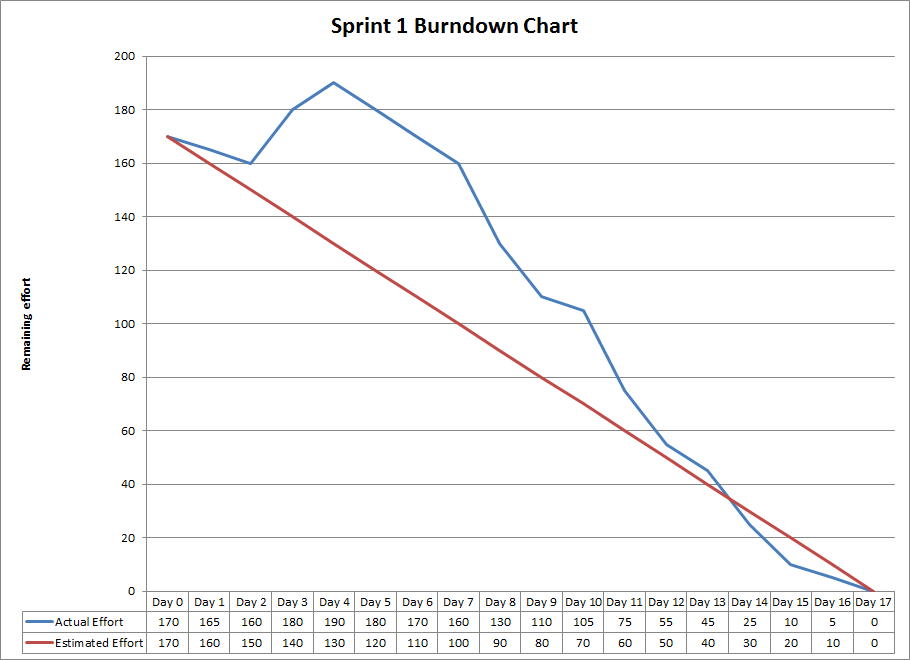
\includegraphics[width=0.5\textwidth]{images/burndown.png} % Image
    \caption{Example sprint burn down chart} % Caption
\end{figure}

\subsubsection{Sprint Retrospective}
At the end of each sprint there will be a meeting to discuss accomplishments, failures, and effort expended. 

\subsubsection{Individual Status Reports}
Statuses for each team member will be their completed tasks and how far into completion they are on unfinished tasks. These status reports will be given to the entire group, and notes and updates made to our Jira board accordingly by Evan Cornish.

\subsubsection{Engineering Notebooks}
engineering notebooks will be updated at a minimum on a weekly basis for each team member. There are 2 sub teams in the beginning for our sprint consisting of Evan and Zach on subteam A and Kartikey, Osama and Paola on subteam B. Each subteam has a task that can be accomplished in parallel. As such each member from either subteam can sign off as a witness for that same members engineering notebook.

\subsection{Closeout Materials}


\subsubsection{System Prototype}
The final system prototype will include a working tethered underwater robot capable of all kinds of movements ranging from forward, backward, sideways to sinking down to bottom and rising to the surface of a water body. The final prototype will also include a display of mechanism capable of collecting trash and dropping it at a desired place.  

The offsite demonstration will take place at the IEEE robotics competition in Houston.  

\subsubsection{Project Poster}
The project poster will include an animated picture of the robot highlighting the thrusters and trash collecting mechanism with animated picture of all team members standing around it in a testing field.  

The project poster will be delivered by UTA Innovation Day.

\subsubsection{Web Page}
The web page will include the project poster, introduction of the project along with IEEE robotics competition introduction, and a segment with team member's introductions. It will be made available to public along with updates on the making of this underwater robot. The webpage will me made available throughout the project and will be delivered by the end of $3^{rd}$ sprint cycle.  

\subsubsection{Demo Video}
The demo video will include the robot successfully moving through three rings of different diameters (first one being largest and last one being smallest) at bottom of a pool. Furthermore, the robot will be seen collecting trash box and bringing it to a platform on the surface of the said pool.  

The length of video will range anywhere from 15 to 30 minutes depending on the power provided to the robot.  

\subsubsection{Source Code}
The team has decided to use GitHub as version control system to maintain source code. The source code will be delivered to binaries only. After the competition is concluded the source code will be made available to the public under the MIT license. The terms will be listed at the top of each source code file.  

\subsubsection{Source Code Documentation}
The team will use Doxygen to generate source code documentation. The final documentation will be provided in browsable HTML format.  

\subsubsection{Hardware Schematics}
The hardware schematics is still a topic of discussion, and nothing is confirmed as of now. The team is considering using a Raspberry pi and Arduino Microcontroller to control the thrusters and camera and wire them up with the system control.  

This section will be updated in the next sprint cycle.  

\subsubsection{CAD files}
This project will involve mechanical design and a 3D printer will be used to print certain components for the mechanical frame of the robot.  

The team will use software named 'tinkercad' to generate files for 3D printing and the file format provided in the closeout material will be STL.  

\subsubsection{Installation Scripts}
Not applicable  

\subsubsection{User Manual}
Since this project is for a robotics competition and the team will do a live demonstration of the robot and its capabilities, a user manual won't be provided or necessary.  

\newpage

%%% References
\bibliographystyle{plain}
\bibliographystyle{reference/IEEEtran_custom}
\bibliography{reference/refs}{}

\end{document}